\mySection{6.4  Type I and Type II Errors}
%-------------- start slide -------------------------------%{{{ 1
\begin{frame}[fragile]
\begin{center}
 \renewcommand{\arraystretch}{2.5}
 \begin{tabular}{c|c|c|}
   &  \multicolumn{2}{|c|}{True State of Nature} \\ \cline{2-3}
      &$H_0$ is true & $H_1$ is true\\
%    \cline{2-3}
  \hline
   Fail to reject $H_0$ & \textcolor{green}{Correct} & \textcolor{magenta}{Type II error}\\
  \cline{2-3}
   Reject $H_0$ & \textcolor{red}{Type I error} & \textcolor{green}{Correct}\\
  \hline
 \end{tabular}
\end{center}
\end{frame}
%-------------- end slide -------------------------------%}}}
%-------------- start slide -------------------------------%{{{ 6.20
\begin{frame}
  % {\S\: 6.4  Type I and Type II Errors}
\begin{center}
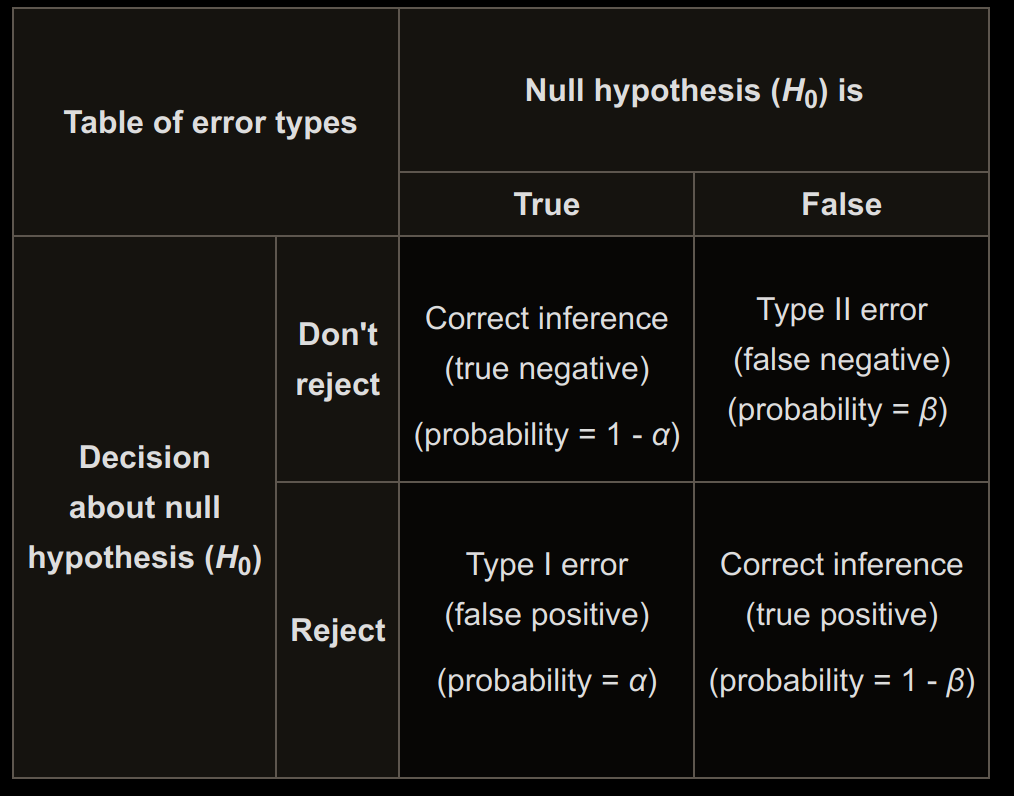
\includegraphics[scale=0.23]{TypeI-II-neg.png}
\end{center}
\end{frame}
%-------------- end slide -------------------------------%}}}
%-------------- start slide -------------------------------%{{{ 6.21
\begin{frame}{Type I error $\sim \alpha$}

 \[
   \alpha:=\bbP(\text{\textcolor{red}{Type I error}}) = \PP(\text{Reject $H_0$}| \text{$H_0$ is true})
 \]
 \vfill\pause
 By convention, $H_0$ is always of the form, e.g.,  $\mu=\mu_0$. So this probability can be exactly determined. It is equal to the level of significance $\alpha$.\\[1em]
 (Simple null test)
\end{frame}
%-------------- end slide -------------------------------%}}}
%-------------- start slide -------------------------------%{{{ 6.22
\begin{frame}{Type II error $\sim \beta$}
 \[
   \beta:=\PP(\text{\textcolor{magenta}{Type II error}}) = \PP(\text{Fail to reject $H_0$}| \text{$H_1$ is true})
 \]
 \vfill\pause
 In order to compute Type II error, we need to specify a concrete alternative hypothesis.
 \vfill
\begin{figure}
 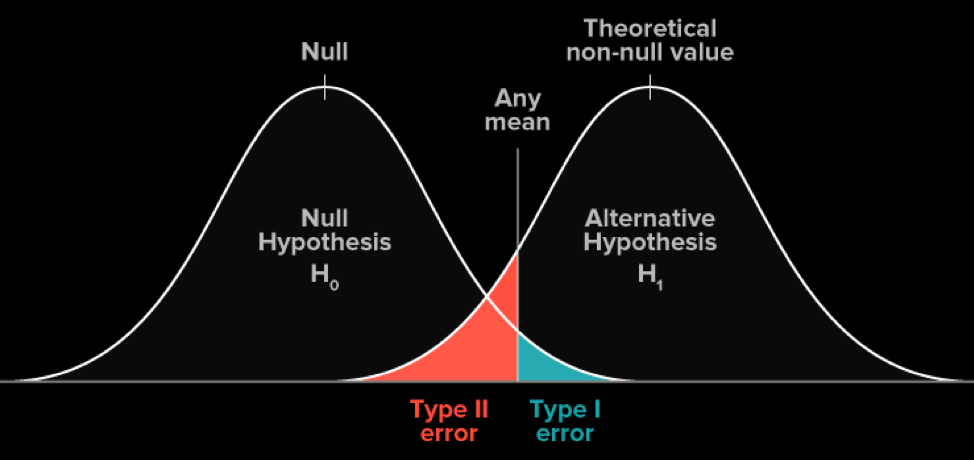
\includegraphics[scale=0.45]{alpha-beta-neg.png}
 \caption{One-sided inference $H_1: \mu>\mu_0$}
\end{figure}

\end{frame}
%-------------- end slide -------------------------------%}}}
%-------------- start slide -------------------------------%{{{ 6.23
\begin{frame}
\begin{figure}
 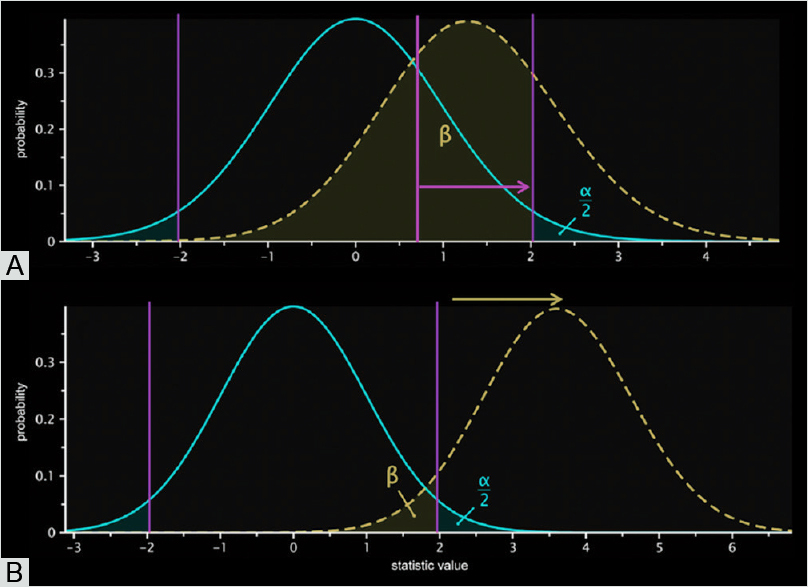
\includegraphics{alpha-2beta-neg.jpg}
 \caption{Two-sided inference $H_1: \mu\ne \mu_0$}
 \end{figure}
\end{frame}
%-------------- end slide -------------------------------%}}}
%-------------- start slide -------------------------------%{{{ 6.24
\begin{frame}{Power of test $1-\beta$}
 \[
 \text{Power of test} = \PP(\text{Reject $H_0$}| \text{$H_1$ is true}) = 1-\beta
 \]
 \vfill
 \begin{center}
  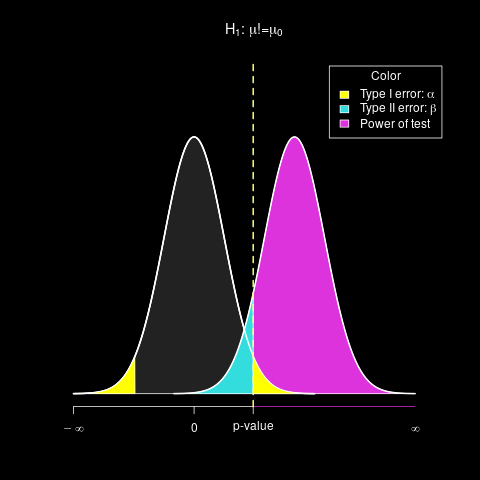
\includegraphics[scale=0.32]{Type-I-II-TwoSided-neg.png}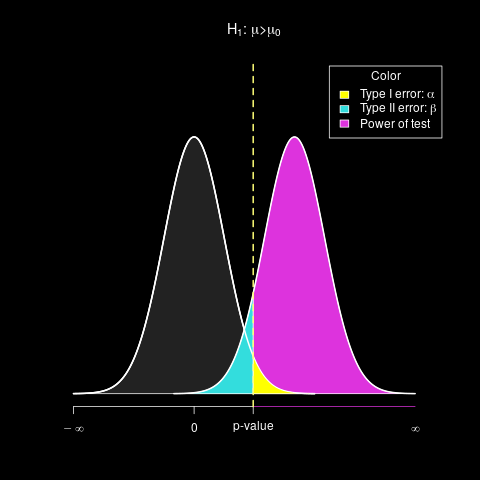
\includegraphics[scale=0.32]{Type-I-II-OneSided-neg.png}
%   \caption{One-sided test $H_1: \mu>\mu_0$}
 \end{center}
 \vfill
 \centering
 One online interactive show all $\alpha$, $\beta$ and $1-\beta$:\\
 \url{https://rpsychologist.com/d3/NHST/}
\end{frame}
%-------------- end slide -------------------------------%}}}
%-------------- start slide -------------------------------%{{{ 6.25
\begin{frame}{Two-sided test}
\def\a{0.27}
 \begin{overlayarea}{\textwidth}{\textheight}
 \begin{center}
	 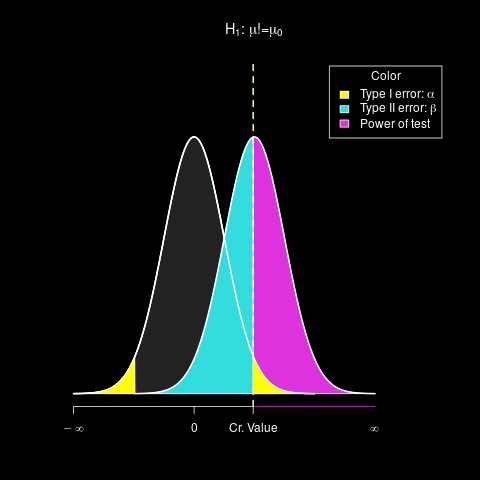
\includegraphics[scale=\a]{Type-I-II-TwoSided-2-neg.png}
	 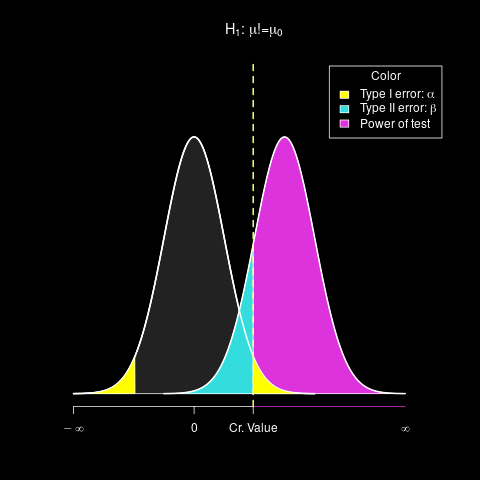
\includegraphics[scale=\a]{Type-I-II-TwoSided-3-neg.png}
	 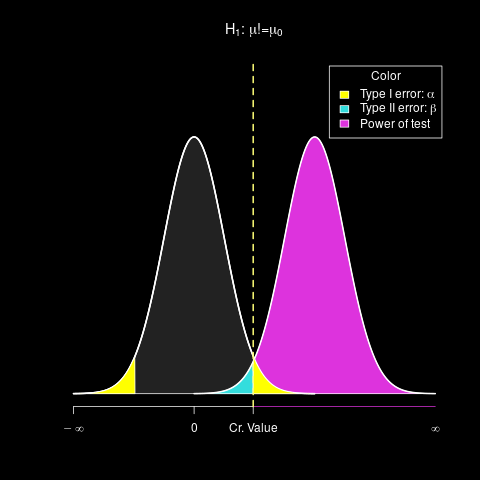
\includegraphics[scale=\a]{Type-I-II-TwoSided-4-neg.png}
 \end{center}
 \end{overlayarea}
\end{frame}
%-------------- end slide -------------------------------%}}}
%-------------- start slide -------------------------------%{{{ 6.26
\begin{frame}{One-sided test}
\def\a{0.27}
 \begin{overlayarea}{\textwidth}{\textheight}
 \begin{center}
	 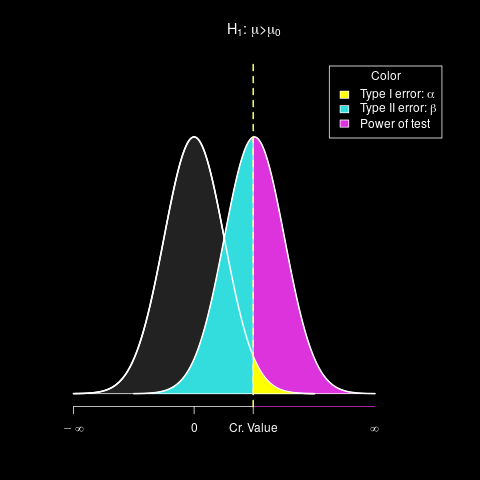
\includegraphics[scale=\a]{Type-I-II-OneSided-2-neg.png}
	 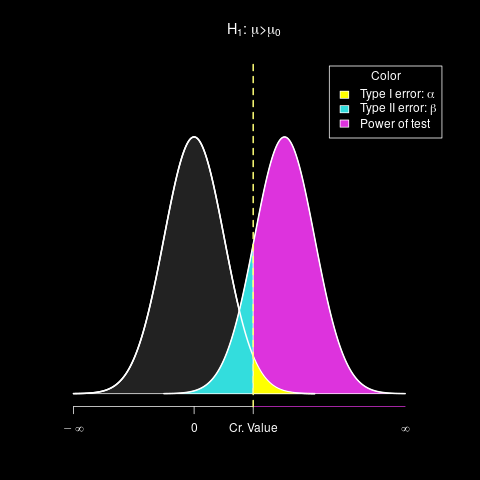
\includegraphics[scale=\a]{Type-I-II-OneSided-3-neg.png}
	 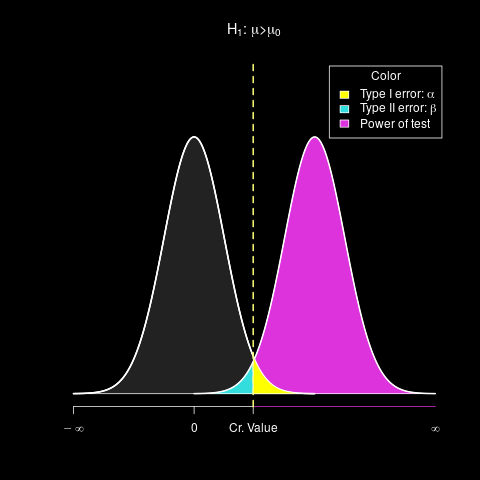
\includegraphics[scale=\a]{Type-I-II-OneSided-4-neg.png}
 \end{center}
 \end{overlayarea}
\end{frame}
%-------------- end slide -------------------------------%}}}
%-------------- start slide -------------------------------%{{{ 6.27
\begin{frame}
 \centering
 Use the {\bf power curves} to select methods \\
 (steepest one!)
 \vfill
 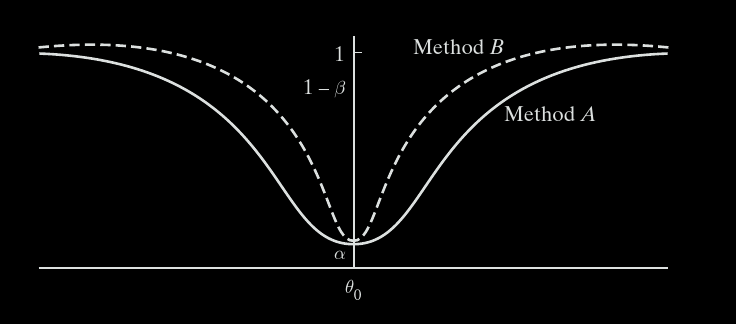
\includegraphics[scale=0.3]{Figure-6-4-5-neg.png}
\end{frame}
%-------------- end slide -------------------------------%}}}
%-------------- start slide -------------------------------%{{{ 6.28
\begin{frame}
 \centering
  $\alpha\uparrow \quad \Longrightarrow\quad \beta\downarrow \quad\text{and}\quad (1-\beta)\uparrow$
  \vfill
 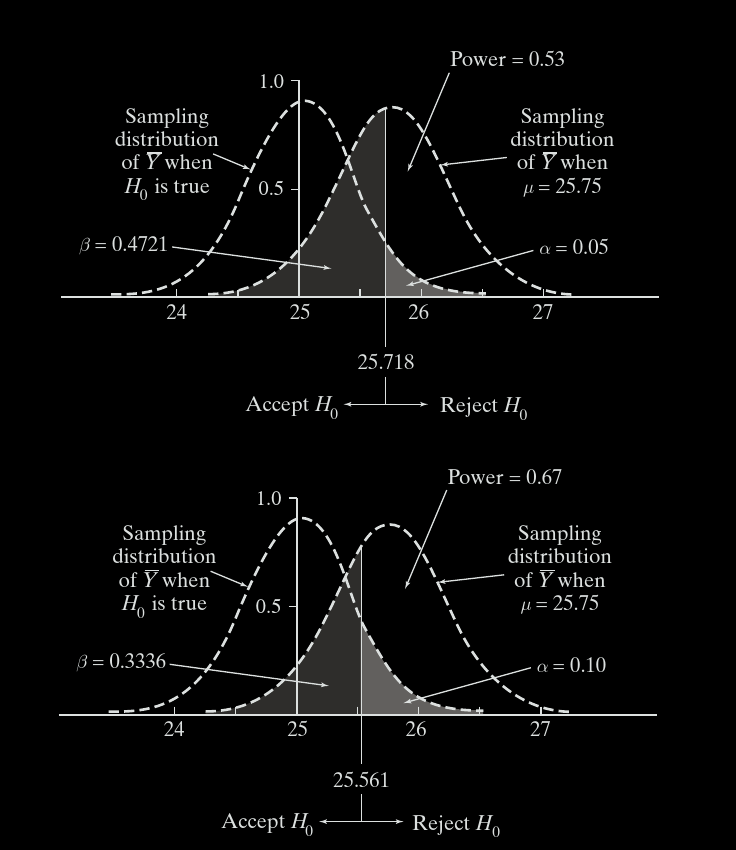
\includegraphics[scale=0.3]{Figure-6-4-6-neg.png}
\end{frame}
%-------------- end slide -------------------------------%}}}
%-------------- start slide -------------------------------%{{{ 6.29
\begin{frame}
 \centering
  $\sigma\downarrow \quad \Longrightarrow\quad \beta\downarrow \quad\text{and}\quad (1-\beta)\uparrow$
  \vfill
 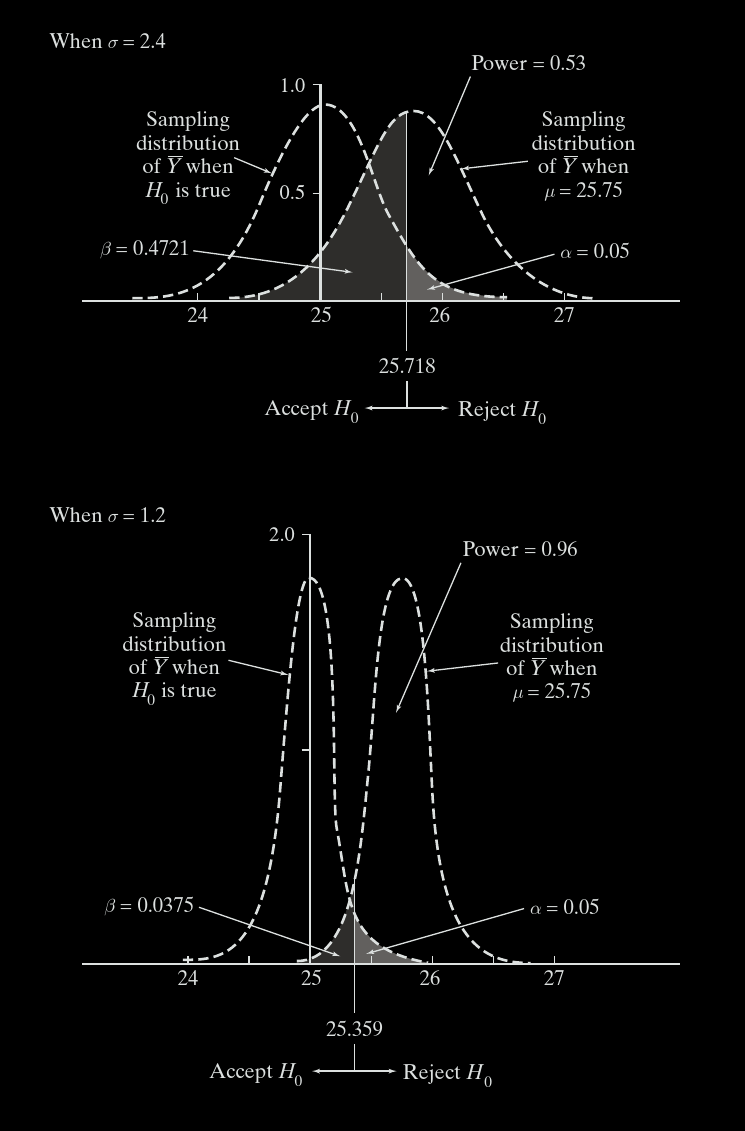
\includegraphics[scale=0.23]{Figure-6-4-7-neg.png}
\end{frame}
%-------------- end slide -------------------------------%}}}
%-------------- start slide -------------------------------%{{{ 6.30
\begin{frame}
 One usually cannot control the given parameter $\sigma$. But one can achieve the same power of test by increasing the sample size $n$.
 \vfill\pause
 \begin{enumerate}
% Example 6.4.1 ...
  \item[E.g. ] Test $H_0:\mu=100$ v.s. $H_1:\mu>100$ at $\alpha=0.05$ with $\sigma=14$ known.\\
	  Requirement: $1-\beta = 0.60$ when $\mu=103$.\\
	  Find smallest sample size $n$. \\[1em]\pause
	  Remark: Two condisions: $\alpha=0.05$ and $1-\beta=0.60$\\
	  \hspace{4.1em}Two unknowns: Critical value $y^*$ and sample size $n$
	  \vfill
  \item[Sol.]
\begin{align*}
C=&
\left\{
z: z = \frac{\bar{y}-\mu_0}{\sigma/\sqrt{n}}\ge z_{\alpha}
\right\}.
\end{align*}
 \end{enumerate}
\end{frame}
%-------------- end slide -------------------------------%}}}
%-------------- start slide -------------------------------%{{{ 6.31
\begin{frame}
	\begin{enumerate}
		\item[]
		\begin{align*}
	1-\beta & =\bbP\left(\frac{\overline{Y}-\mu_0}{\sigma/\sqrt{n}}\ge z_{\alpha} \:\bigg|\mu_1\right)\\\pause
& =
\bbP\left(\frac{\overline{Y}-\mu_1}{\sigma/\sqrt{n}} + \frac{\mu_1-\mu_0}{\sigma/\sqrt{n}}\ge z_{\alpha} \:\bigg|\mu_1\right)\\\pause
&=
\bbP\left(Z\ge  - \frac{\mu_1-\mu_0}{\sigma/\sqrt{n}}+ z_{\alpha} \:\bigg|\mu_1\right)\\\pause
&=\Phi\left( \frac{\mu_1-\mu_0}{\sigma/\sqrt{n}}- z_{\alpha} \right)
\end{align*}\pause
\[
	\frac{\mu_1-\mu_0}{\sigma/\sqrt{n}}- z_{\alpha}  = \Phi^{-1}(1-\beta)
	\quad\Longleftrightarrow\quad
	n = \left(\sigma\times \frac{\Phi^{-1}(1-\beta) + z_{\alpha}}{\mu_1-\mu_0}\right)^2
\]\pause
\[
	n = \Ceil{\left(14\times \frac{0.2533+1.645}{103-100}\right)^2} =\Ceil{78.48} = 79.
\]
\myEnd
\end{enumerate}
\vfill
\begin{minipage}{0.34\textwidth}
\begin{center}
\small
 R\\
 $z_\alpha = \text{qnorm}(1-\alpha)$ \\
 $\Phi^{-1}(1-\beta) = \text{qnorm}(1-\beta)$
\end{center}
\end{minipage}
\begin{minipage}{0.64\textwidth}
\begin{center}
\small
 Python\\
$z_\alpha = \text{scipy.stats.norm.ppf}(1-\alpha)$ \\
$\Phi^{-1}(1-\beta) = \text{scipy.stats.norm.ppf}(1-\beta)$
\end{center}
\end{minipage}
\end{frame}
%-------------- end slide -------------------------------%}}}
%-------------- start slide -------------------------------%{{{ 6.32
\begin{frame}{Nonnormal data}
	Test $H_0:\theta = \theta_0$, with $f_Y(y;\theta)$ is not normal distribution. \pause
	\vfill
	\begin{enumerate}
		\item Identify a sufficient estimator $\widehat\theta$ for $\theta$
			\vfill
		\item Find the critical region $C$:  Least compatible with $H_0$ but \\
			\hspace{12em} still admissible under $H_1$
			\vfill
		\item Three types of questions:
    \item[] Given $\alpha$ $\rightarrow$ find $C$ \pause $\rightarrow$ $\beta$, $1-\beta$...\\
		\item[] From $C$  $\rightarrow$ determine $\alpha$ \\
		\item[] From $\theta_e$ $\rightarrow$ find $P$-value
	\end{enumerate}
\end{frame}
%-------------- end slide -------------------------------%}}}
%-------------- start slide -------------------------------%{{{ 6.33
\begin{frame}{Examples for nonnormal data}

 \begin{enumerate}
	 \item[E.g. 1.] A random sample of size $n$ from \underline{uniform distr.}
		 $f_Y(y;\theta)=1/\theta$, $y\in[0,\theta]$. To test
		 \[
			 H_0:\theta=2.0 \quad\text{v.s.}\quad H_1: \theta<2.0
		 \]
		 at the level $\alpha=0.10$ of significance, one can use the decision rule based on
		 $Y_{max}$. Find the probability of committing a Type II error when $\theta=1.7$.\\[1em]
		 Remark: $Y_{max}$ is a sufficient estimator for $\theta$. Why?
	\pause	 \vfill
\item[Sol.]
	 1) The critical region should has the form: $C=\{y_{max}: y_{max}\le c\}$. \\[1em] \pause
		2) We need to use the condition $\alpha=0.10$ to find $c$.\\[1em] \pause
		3) Find the prob. of Type II error.
 \end{enumerate}

\end{frame}
%-------------- end slide -------------------------------%}}}
%-------------- start slide -------------------------------%{{{ 6.34
\begin{frame}
	\begin{center}
 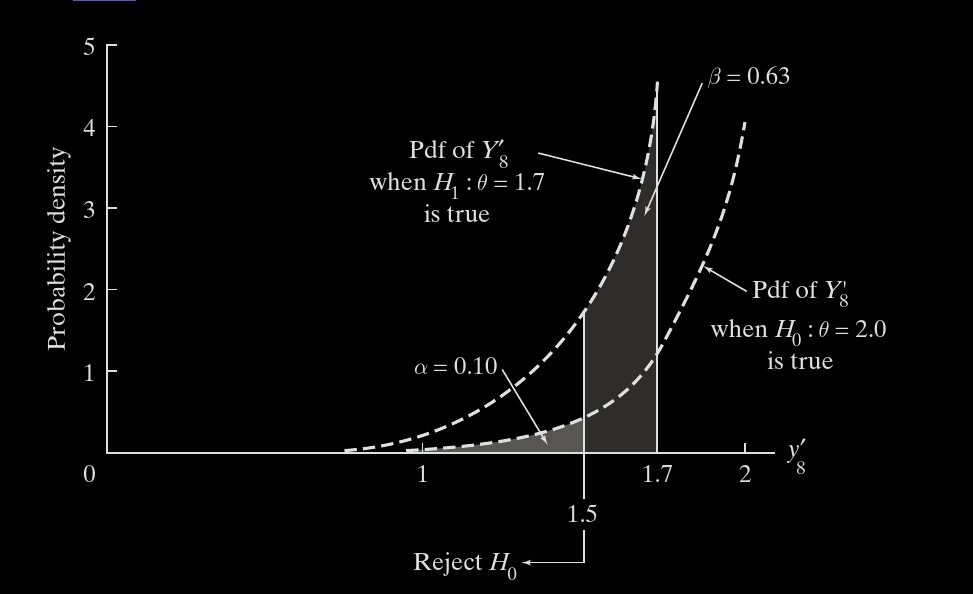
\includegraphics[scale=0.23]{Figure-6-4-8-neg.png}
	\end{center}
\[
	f_{Y_{max}}(y) = ... = n\frac{y^{n-1}}{\theta^n} \quad y\in[0,\theta].
\]
\begin{align}\tag{Under $H_0:\theta=\theta_0$}
	\alpha = \int_0^c n\frac{y^{n-1}}{\theta_0^n}\ud y = \left( \frac{c}{\theta_0} \right)^n \quad \Longrightarrow\quad  c= \theta_0\alpha^{1/n}
\end{align}
\begin{align}\tag{Under $\theta=\theta_1$}
\beta = \int_{\theta_0\alpha^{1/n}}^{\theta_1} n\frac{y^{n-1}}{\theta_1^n}\ud y
 = 1- \left(\frac{\theta_0}{\theta_1}\right)^n \alpha
\end{align}
Finally, we need only plug in the values $\theta_0=2$, $\theta_1=1.7$ and $\alpha=0.10$.
\myEnd
\end{frame}
%-------------- end slide -------------------------------%}}}
%-------------- start slide -------------------------------%{{{ 6.35
\begin{frame}
	\begin{enumerate}
		\item[E.g. 2.] A random sample of size $4$ from Poisson$(\lambda)$: $p_X(k;\lambda)=e^{-\lambda}\lambda^k/k!$, $k=0,1,\cdots$.
			One wants to test
			\[
				H_0:\lambda=0.8 \quad\text{v.s.}\quad
				H_1:\lambda>0.8.
			\]
			at the level $\alpha=0.10$. Find power of test when $\lambda=1.2$.
			\vfill
		\item[Sol.] 1) We've seen: $\overline{X}=\sum_{i=1}^4 X_i$ is a sufficent estimator for $\lambda$;\\
    \begin{align*}
      \overline{X}\sim\text{Poisson}(3.2)
    \end{align*}
			\pause
			2) $C=\{\bar{k};\bar{k}\ge c\}$. \\[1em]\pause
			3) $\alpha=0.10$ $\rightarrow$ $c=6$. \\[1em]\pause
			4) Alternative $\lambda=1.2$ $\rightarrow$ $1-\beta = 0.35$.
	\end{enumerate}
\end{frame}
%-------------- end slide -------------------------------%}}}
%-------------- start slide -------------------------------%{{{ 6.36
\begin{frame}[fragile]
\begin{center}
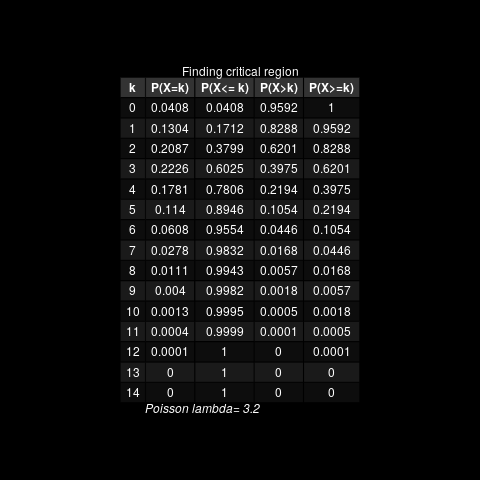
\includegraphics[scale=0.45]{Example_6-4-3_1-neg.png}
\vfill

\begin{minipage}{0.25\textwidth}
\begin{center}
\begin{lstlisting}[language=R]
> qpois(1-0.10,3.2)
[1] 6
\end{lstlisting}
\end{center}
\end{minipage}
\quad
\begin{minipage}{0.5\textwidth}
\begin{center}
\begin{lstlisting}[language=Python]
> scipy.stats.poisson.ppf(1-0.10,3.2)
[1] 6
\end{lstlisting}
\end{center}
\end{minipage}
\end{center}
\end{frame}
%-------------- end slide -------------------------------%}}}
%-------------- start slide -------------------------------%{{{ 6.37
\begin{frame}[fragile]
\begin{center}
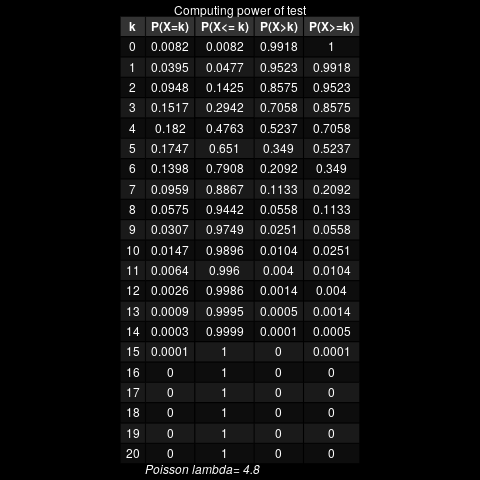
\includegraphics[scale=0.38]{Example_6-4-3_2-neg.png}
\[
	1-\beta = \bbP\left(\text{Reject $H_0$}\mid \text{$H_1$ is true}\right)
	=\bbP(\overline{X}\ge 6|\overline{X}\sim Poisson(4.8))
\]
\myEnd
\bigskip

\begin{minipage}{0.25\textwidth}
\begin{center}
\begin{lstlisting}[language=R]
> 1-ppois(6-1,4.8)
[1] 0.3489936
\end{lstlisting}
\end{center}
\end{minipage}
\qquad
\begin{minipage}{0.45\textwidth}
\begin{center}
\begin{lstlisting}[language=Python]
> 1-scipy.stats.poisson.cdf(6-1,4.8)
[1] 0.3489935627305083
\end{lstlisting}
\end{center}
\end{minipage}
\end{center}
\end{frame}
%-------------- end slide -------------------------------%}}}
%-------------- start slide -------------------------------%{{{ 6.38
\begin{frame}[fragile]
\begin{lstlisting}[title=The {\it R} code to produce the previous two Poisson tables.]
PlotPoissonTable <- function(n=14,lambda=3.2,png_filename,TableTitle) {
  library(gridExtra)
  library(grid)
  library(gtable)
  x = seq(1,n,1)
  # qpois(0.90,lambda)
  tb = cbind(x,
             round(dpois(x,lambda),4),
             round(ppois(x,lambda),4),
             round(1-ppois(x,lambda),4),
             round(c(1,(1-ppois(x,lambda))[1:n]),4))
  colnames(tb) <- c("k", "P(X=k)", "P(X<= k)", "P(X>k)", "P(X>=k)")
  rownames(tb) <-x
  table <- tableGrob(tb,rows = NULL)
  title <- textGrob(TableTitle,gp=gpar(fontsize=12))
  footnote <- textGrob(paste("Poisson lambda=",lambda),
                       x=0, hjust=0, gp=gpar( fontface="italic"))
  padding <- unit(0.2,"line")
  table <- gtable_add_rows(table, heights = grobHeight(title) + padding,pos = 0)
  table <- gtable_add_rows(table, heights = grobHeight(footnote)+ padding)
  table <- gtable_add_grob(table, list(title, footnote),
                           t=c(1, nrow(table)), l=c(1,2),r=ncol(table))
  png(png_filename)
  grid.draw(table)
  dev.off()
}

PlotPoissonTable(14,3.2,"Example_6-4-3_1.png","Finding critical region")
PlotPoissonTable(20,4.8,"Example_6-4-3_2.png","Computing power of test")
\end{lstlisting}
\end{frame}
%-------------- end slide -------------------------------%}}}
%-------------- start slide -------------------------------%{{{ 6.39
\begin{frame}[fragile]
\begin{enumerate}
	\item[E.g. 3.] A random sample of size $7$ from $f_Y(y;\theta)=(\theta+1)y^\theta$, $y\in[0,1]$.
		Test
		\[
			 H_0:\theta=2.0 \quad\text{v.s.}\quad H_1: \theta>2.0
		\]
		Decision rule: Let $X$ be the number of $y_i$'s that exceed $0.9$; \\
    \phantom{Decision rule:} Reject $H_0$ if $X\ge 4$. \\
		Find $\alpha$.
		\pause
    \bigskip
	\item[Sol.] 1) $X\sim$ binomial$(7,p)$. \\ \pause
		2) Find $p$:
		\begin{align*}
			p&=\bbP(Y\ge 0.9| \text{$H_0$ is true}) \\
			 &= \int_{0.9}^1 3y^2 \ud y = 0.271
		\end{align*}\pause
		3) Compute $\alpha$:
		\[
			\alpha=\bbP(X\ge 4|\theta=2) = \sum_{k=4}^7 {7\choose k} 0.271^k 0.729^{7-k}
			=0.092.
		\]
    \myEnd
\end{enumerate}
\begin{center}
\begin{minipage}{0.3\textwidth}
\begin{center}
\begin{lstlisting}[language=R]
> 1-pbinom(3,7,0.271)
[1] 0.09157663
\end{lstlisting}
\end{center}
\end{minipage}
\quad
\begin{minipage}{0.5\textwidth}
\begin{center}
\begin{lstlisting}[language=Python]
> 1-scipy.stats.binom.cdf(3, 7, 0.271)
[1] 0.09157663095582469
\end{lstlisting}
\end{center}
\end{minipage}
\end{center}
\end{frame}
%-------------- end slide -------------------------------%}}}

